\section{Optimizing the LS$^{2}$ simulation engine}
\label{Implementation}
In the following section I will describe how I optimized the LS$^{2}$ simulation engine using mainly SSE intrinsics. I will begin introducing the software itself and its research purpose. Then, I will document the approach taken for development, including information about how I benchmarked the application in order to acquire meaningful results. The main part of this section will comprise an overview of the optimized source codes of the three algorithms that I have chosen to improve. Code sections of particular interest with regards to special SSE programming techniques will be singled out and explained in detail.

\subsection{LS$^{2}$: A simulation engine for lateration algorithms}
\label{ls2}
The term ``lateration algorithms'' is commonly used to refer to geometric algorithms that use distance measurements to determine the location of points in the plane or in a three-dimensional space (as opposed to triangulation which uses the measurement of angles). The most basic representative of this group of algorithms is known as \emph{Trilateration}: Obviously, in the euclidean plane it needs at least three known spots (subsequently called \emph{anchors}) and the distance measurements hereof to be able to narrow down the current position to a single point. Relative to each of the anchors, this point lies on a circle that has its center on the anchor and the distance as its radius. Trilateration determines the current position by solving these three linear equations, in other words, it calculates the intersection of the three circles drawn around the anchors. In real-world applications such as the Global Positioning System (GPS) or indoor localization, distance measurements, like all physically measured data, are generally error-prone. Most commonly, distances are estimated by measuring the time it takes a signal (e.g. light, radio) to travel between an anchor and the client. Because of these erroneous distances, circles drawn around the anchors do not necessarily intersect at a single point and the basic trilateration algorithm fails to produce an exact result. In order to calculate an approximation of the current position, trilateration can be adapted to return the geometric center of the now up to three circle intersections. However, during the last decades, several superior, more complex algorithms have been found that compute improved position estimations based on error-prone distances of three or more anchors.

The \emph{FU Berlin Parallel Lateration-Algorithm Simulation and Visualization Engine} (LS$^{2}$), written by Heiko Will, Thomas Hillebrandt, and Marcel Kyas and first presented at the WPNC conference 2012, is a graphical evaluation framework for lateration algorithms. As the authors explain in~\cite{will2012ls2}, the application's fundamental idea is to not only calculate an average algorithm error based on randomized locations, which has been the main evaluation criterium for lateration algorithms so far, but to calculate errors for all locations on a given ``playing field'' in parallel and in the end to provide the user with an image displaying the so-called \emph{spatial position error distribution}. The assumption is that the position of the anchors has significant influence on the algorithm's performance, even more so than the errors of the distances. Figure~\ref{fig:lateration} shows an exemplary output image created with the LS$^{2}$ engine using the VBLE-OPT algorithm and a set of 3 anchors, only the anchor positions have been slighty magnified for better visibility. The left part of the image displays the average position error for every location (where bright colors indicate low average error), whereas part to the right displays the highest error for every position.

\begin{figure}[ht]
\begin{center}
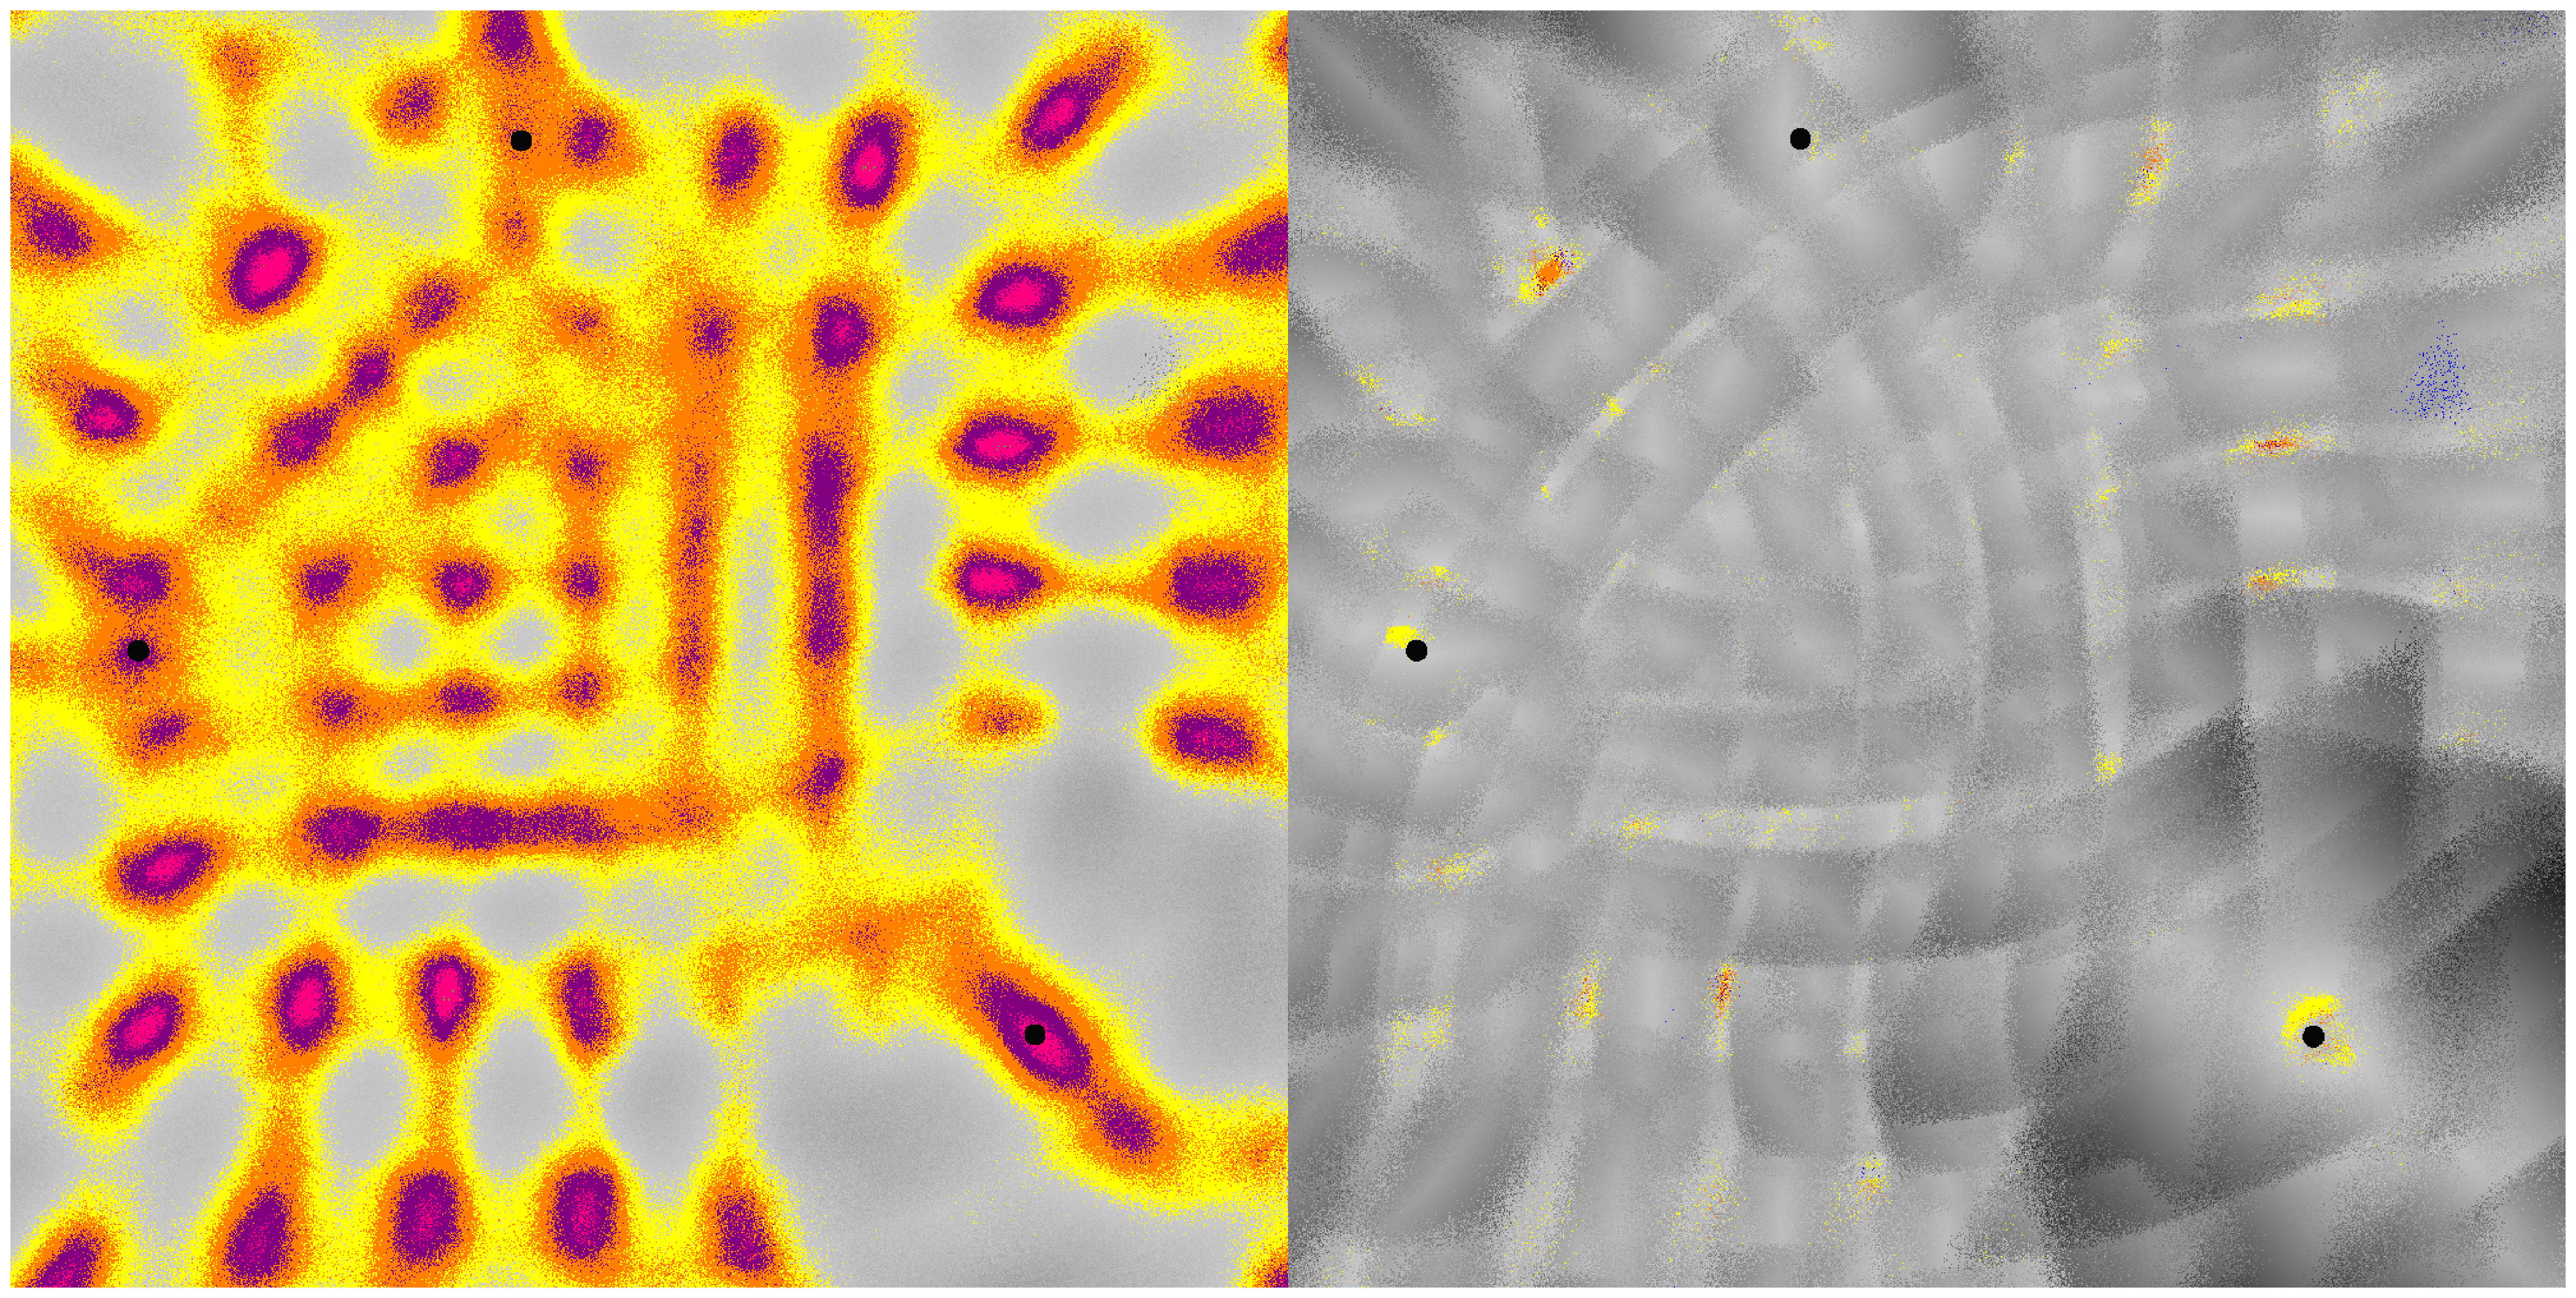
\includegraphics[width=14cm]{img/lateration}
\end{center}
\caption{Example output of the LS$^{2}$ engine}
\label{fig:lateration}
\end{figure}

The application is divided into three main parts: The engine itself, responsible for distributing the work load and calculating the position errors, a set of error models, which are used to simulate the distance measurement errors, and the lateration algorithms. Parametrized with a set of anchor positions, the error model, and the desired algorithm, the engine first starts a number of threads and associates them with a spatial slice of the 1000x1000 playing field. For each position in its slice, a thread calculates the real distance between the position and the anchors, randomly modifies the distances according to the error model, and executes the lateration algorithm. It then calculates the algorithm error as the difference between the real distance and the algorithm's return value. This process is repeated for a configurable number of iterations (defaults to 1000) for each position, before the resulting average error is written back to an image buffer. At the time of writing, LS$^{2}$ features 6 different lateration algorithms, of which 4 are standard algorithms such as trilateration or \emph{Adapted Multilateration} (AML) and 2 are novel algorithms provided by the authors themselves. Regarding the error model, the user can choose between a uniform distribution and a Gaussian distribution of error values, although work is underway to support map-based error models as well.

The LS$^{2}$ engine is implemented in C99 dialect and is thoroughly optimized for speed. All functions are forcibly inlined and reside in the same compilation unit. Apart from the image buffer, no dynamically allocated memory is used. The engine itself uses SSE instructions or, at the user's wish, the newer AVX instructions available on Intel's most recent Sandy Bridge microprocessors, to process 4 respectivly 8 iterations at once. For example, the calculation of the true distances is fully vectorized as is the random number generator used by the error models. Afterwards, the engine will execute the user-requested lateration algorithm with vectorized parameters. To understand the mechanics, refer to Listing~\ref{prototype} which shows the function definition of the trilateration algorithm. The \texttt{count} parameter specifies the number of anchors the algorithm should use, whose x- and y-coordinates are contained in the \texttt{vx} and \texttt{vy} arrays. Note, that these, as well as the distance array \texttt{r} and the result buffers \texttt{resx} and \texttt{resy}, are declared as \texttt{VECTOR}s, which means that there are 4 (resp. 8) of each of these values waiting to be processed at once. Note that \texttt{VECTOR} is a preprocessor \texttt{define} mapping to \texttt{\_\_mm128} when the application is compiled in SSE mode and to \texttt{\_\_mm256} in AVX mode.

\begin{code}[caption={Prototype of the \texttt{trilaterate} function},label=prototype]
void trilaterate(const int count, const VECTOR* vx, 
                 const VECTOR* vy, const VECTOR* r, 
                 VECTOR* resx, VECTOR* resy);
\end{code}

When I started looking into optimizing the LS$^{2}$ application for this thesis, some algorithms shipped with it, for example trilateration and the \emph{Linear Least Squares} algorithm, already made use of SSE instructions to process their parameters in a single run. Yet, some others were merely literal transcriptions from a scalar implementation and were not aware of vector processing at all. These algorithms (\emph{Geolateration}, \emph{Optimized Voting Based Location Estimation}, and \emph{Adapted Multilateration}) simply unwrapped the vectors at the function head, calculated the position estimations in scalar code, and packed the results back into the result buffers at the end of the function. Therefore, these three algorithms best qualified for having a deeper look into their optimization potential.

\subsection{Development approach}
During the development period, it quickly became clear to me that software optimization is not an utterly straightforward task, but instead is a rather non-linear process involving mostly trial and error methods. Quite often attempting to optimize a particular piece of code using a specific optimization technique would not lead to any performance gains, even though in theory it may have looked like a very promising measure. Yet sometimes, these attempts that seemed to be ``dead-ends'' at first try later became valuable complements to other optimization efforts. As a consequence, my ``development process'', which was anything but well-defined at the beginning, turned out to be slightly different from regular iterative processes. As it is mainly a report on my personal experiences, the following section should not be misinterpreted as a universal guideline. The described steps and tools simply suited my needs best.

\subsubsection{Determining bottlenecks through profiling}
As Donald E. Knuth has already stated memorably in 1974, it is a good idea to first determine the most performance-critical part of a piece of code before beginning with optimization work, as this is likely the only part where optimization really is worth the effort. To find that critical part, the performance bottleneck, profiling a software can be helpful. For C/C++ code and Unix-like platforms, a tool called \emph{Valgrind}\footnote{\url{http://valgrind.org}, last accessed: \today{}} has become the de-facto standard profiler utility. The Valgrind suite consists of a variety of specialized profiling tools, each of them named differently, as for instance a memory usage analyzer (Mmemcheck) that especially helps finding memory leaks, a heap profiler (Massif) for dynamic memory profiling, and a cache profiler (Cachegrind) that simulates cache utilizitation to detect cache misses. The latter is especially valuable for optimization, as it additionally counts the executed instructions for each code line and is able to estimate the amount of clock cycles the processor needs to execute them. On top of that, Cachegrind features a special option (\texttt{--branch-sim=yes}) that counts branch mispredictions and thus can identify particularly unpredictable branches. Cachegrind's result can be best viewed using the \emph{KCachegrind}\footnote{\url{http://kcachegrind.sourceforge.net/html/Home.html}, last accessed: \today{}} front-end, as demonstrated by the screenshot in Figure~\ref{fig:kcachegrind}.
\begin{figure}[h]
\begin{center}
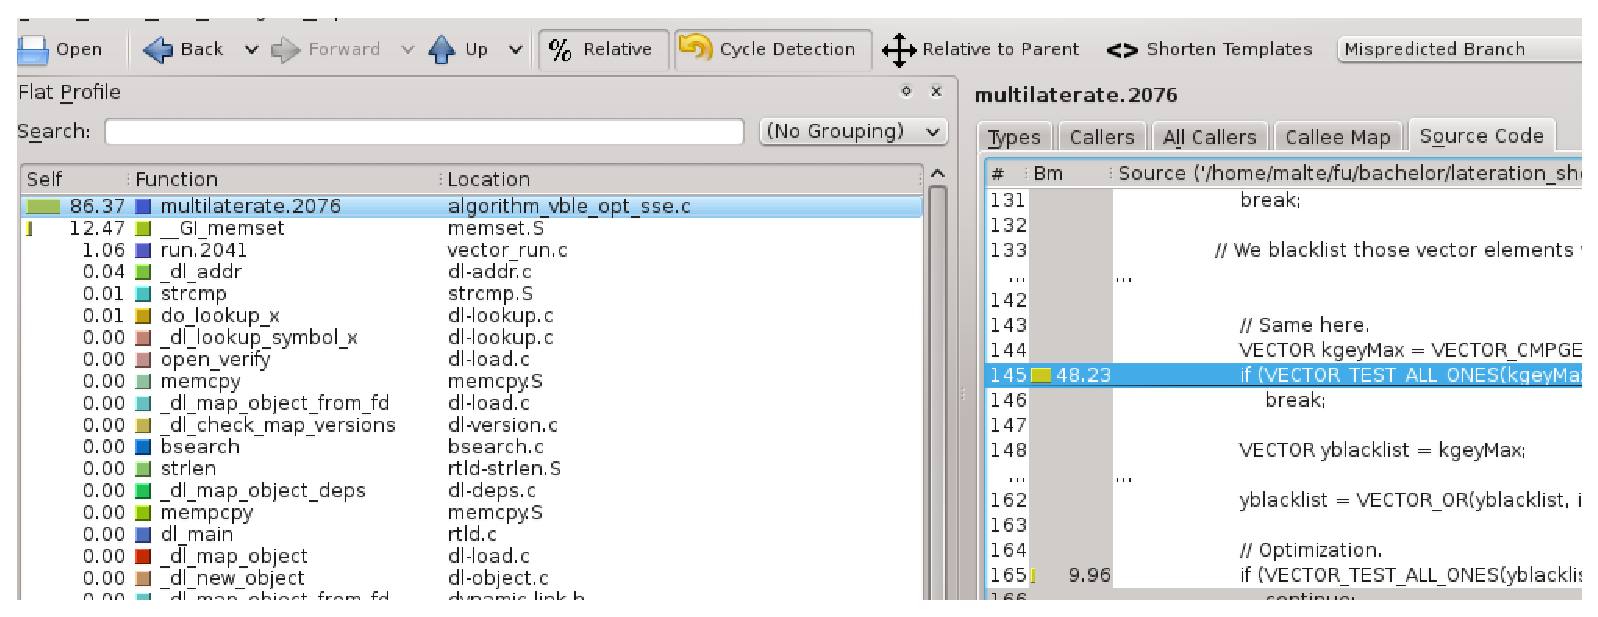
\includegraphics[width=14cm]{img/kcachegrind}
\end{center}
\caption{KCachegrind, branch prediction view}
\label{fig:kcachegrind}
\end{figure}

\subsubsection{Benchmarking optimization efforts}
\label{benchmarking}
After having identified the bottlenecks and resolved them with the help of optimization techniques, the next step is to evaluate their impact on performance. Before and after every smaller step, I used the unix \texttt{time} command to measure performance of the application for a randomly selected set of input values. As can be read on the command's manpage, \texttt{time} measures three different execution times, see Listing~\ref{time} for an example output. The ``user'' value indicates the amount of CPU time spent in user-mode, the ``sys'' value is the amount of CPU time spent in kernel-mode. The ``real'' value is the real time that has elapsed between start and termination of the application. For threaded applications such as LS$^{2}$, on dual-core systems this should ideally be about half of the combined ``user'' and ``sys'' times plus some overhead for context switches. As the ``real'' time varies with the number of processors available and the number of system-calls contained in LS$^{2}$ is close to zero, the only information that made a difference for my optimization work was the ``user'' value.

\begin{shell}[caption={Example output of the unix \texttt{time} command},label=time]
$ time { ./bin/lateration_shooter_sse 100 400 500 200 700 800 ; }
Average error is 45.252751

real    0m8.056s
user    0m14.916s
sys     0m0.008s
$
\end{shell}

As the performance of the various algorithms in LS$^{2}$ turned out to be highly affected by the positions of the anchors, it was also crucial to evaluate the performance gains using a larger amount of randomized input data, in order to avoid optimizing the application for a single case. For this time-consuming task I wrote an increasingly useful Python script called \emph{benchlat}, which automatically compiled my various work states, benchmarked them a larger number of times overnight, and after completion sent me an email containing the analyzed results, namely average and variance of the achieved speed-ups. Individual speed-up ratios were obtained by running the reference implementation and my optimized versions with a the same set of anchor positions. Later I added automatic profiling using Cachegrind as well as an option that allowed tracing the performance fluctuation through the development history. Regarding the selection of anchor positions, I decided to mainly choose points close to (distinct) borders of the playing field. This reduces the bias towards small, centered shapes that would arise from a uniform distribution of points and in general can be considered more realistic for localization scenarios [ZITAT?].

\subsubsection{Managing various attempts using a version control system}
As mentioned before, optimizing LS$^{2}$ was an unsteady task that was characterized by hours of trial and error. When an optimization proved to be the best solution in the very situation and to measurably improve performance, I integrated it into the sources and moved on to the next chokepoint. These successes were often preceded by a number of less profitable attempts that I wanted to save for possible later reuse. Making heavy use of lightweight branches as provided by most modern version control systems such as Git\footnote{\url{http://git-scm.com/}, last accessed: \today{}} proved highly beneficial for these cases. Using branches, I could temporarily put unpromising changes aside and merge them back in when they again seemed practical solutions in combination with other work. To illustrate the trial and error process more vividly, Figure~\ref{fig:branchtree} displays a schematic overview of the development in form of a visualization of the complete Git history. Nodes represent the numerous Git commits, which are linked by arrows indicating an ``ancestor-of'' relationship. As can be seen easily, the development path was not straightforward.

\begin{figure}[h]
\begin{center}
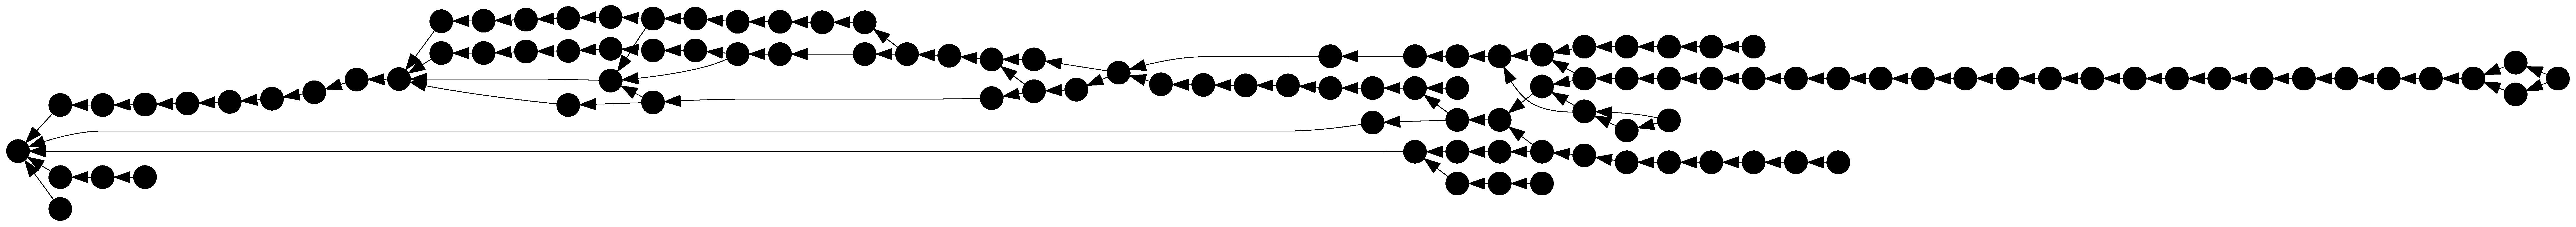
\includegraphics[width=14cm]{img/branchtree}
\end{center}
\caption{Visualization of \texttt{git} history}
\label{fig:branchtree}
\end{figure}

\subsection{Algorithm I: Adapted Multilateration}
Proposed by Kuruoglu et al. in~\cite{kuruoglu2009aml}, Adapted Multilateration (AML) is a lateration algorithm that produces acceptable results while being of lower complexity. Like in the case of tri- and multilateration, it is based on anchor circles and their intersections.

\subsubsection{Functionality}
AML consists of three steps: \emph{intersection and elimination}, \emph{first estimation}, and \emph{refinement}. At the beginning of step 1, two intersecting anchor circles are chosen randomly. If these circles intersect at exactly one point, that point is picked for step 2. In case of two circle intersections, one of them needs to be eliminated, which is the one that has the larger distance to the circle of a third anchor. Afterwards, a first estimation of the position is obtained by moving the intersection point to the middle of the line segment connecting it with the third anchor's circle (i.e. with the closest point on that circle). 
Any remaining anchors are processed in the same way in the final refinement step: For each anchor, the current location estimation is moved to the middle of the shortest line segment connecting it with the anchor's circle. Refer to the paper for a much better and more graphical explanation of the algorithm.

To calculate the said movement, the authors state it would be necessary to differentiate whether the current point is located on the inside or on the outside of the anchor's circle and treat these cases differently. However, I could not spot any reason why this method would be advantageous over using simple vector mathematics\footnote{Let $\vec{p}$ be the vector belonging to the intersection point and $\vec{x}$ the vector pointing at the center of the circle (see figure 3 in~\cite[p. 264]{kuruoglu2009aml}), while $\vec{xp} = \vec{p} - \vec{x}$ is the direction vector from Point $p$ to the center point $x$. We could then determine the intersection $a$ of the line segment between $x$ and $p$ by scaling this direction vector to the circle's radius which means multiplying the vector by $\frac{r}{\left| \vec{xp} \right|}$, i.e. as a vector: $\vec{a} = \vec{x} + \frac{r}{\left| \vec{xp}\right| } \cdot \vec{xp}$. The middle of the line segment $\overline{pa}$ can be calculated as $\vec{p'} = \vec{p} + \frac{1}{2} \cdot \vec{pa} = \vec{p} + \frac{1}{2} \cdot \left( \left( \vec{x} + \frac{r}{\left|\vec{xp}\right|} \cdot \vec{xp} \right) - \vec{p} \right)$.}. Still, as algorithmic optimization was not part of my goals, the optimized code presented in the following corresponds to the author's original algorithm description.

\subsubsection{Optimizations}
Since the AML implementation is concise and easily understood, I will be able to present it in its entirety in this section. For a more generic start, Listing~\ref{circles} displays the already vectorized \texttt{circle\_get\_intersections\_v} function, which, as its name implies, is used to calculate the intersections of two random anchor circles in step 1 of AML, although it is written to process 4 pairs of circles at once, or 8 in the case of AVX. For reference, I included the original scalar implementation of this function in Appendix~\ref{scalarcircles}. The function is based on the usual geometric approach of constructing a line through the intersections and using triangles to determine the offset of the intersections from the line segment connecting the anchors (refer to~\cite{bourke1997circles}) for further explanation). What is most interesting in the SSE implementation, is the treatment of special cases occurring when the circles do not (properly) intersect, of which there are three: First, the circles may be disjunct, i.e. the distance between the anchors is greater than the sum of the circles' radii, second, one circle may be contained within the other (the absolute difference of the radii is less than the distance between the anchors), and third, the anchors may be coincident (the distance is 0), in which case there are 0 or an infinite number of intersections. In the original implementation these special cases were handled by an \texttt{if} statement that contained three boolean expressions linked by logical OR, each of them corresponding to one of the cases. In case the \texttt{if} statement evaluated to \texttt{true}, the function would immediately return 0. To eliminate the conditional jump, the SSE version inverts the boolean expressions and blends the \texttt{retval} vector to 1 in case all expressions are true, 0 otherwise (ll. 11--13 in Listing~\ref{circles}). Afterwards, all the usual calculations are performed regardless of whether the circles contained in the particular vectors truly intersect, which may result in unusual values for vector elements that failed the blending before. For example, coincident anchors, having a distance of 0, will lead to a division by zero in line 15, which results in variable \texttt{a} containing the floating-point-specific value \texttt{+Inf}, or ``positive infinity''. In fact, all intermediary results should be considered ``tainted'' until they are verified by re-checking the mask that is now stored in \texttt{retval}. An example can be seen in line 33: If variable \texttt{h}, which contains the distance between the intersection(s) and the line segment connecting the anchors, is non-zero, the algorithm has found two intersections. In this case, \texttt{retval} is incremented to indicate two solutions, but only when it already holds a 1, in other words, when all special cases have been ruled out. As a noteworthy side-effect to be kept in mind by the programmer, the SSE implementation always modifies the \texttt{resx} and \texttt{resy} vectors, whereas the scalar implementation did not touch them if the circles did not intersect.

\codefile{Calculating circle intersections with SSE}{circles}{code/circles.c}

In order to find two random intersecting anchor circles, the previous implementation of AML simply tried all possible anchor combinations beginning with the first two anchors. However, since it is not guaranteed that the SSE version finds suitable anchor pairs for all vector elements in the same loop iteration, it has to continue the search until this condition is satisfied for all vector elements. Listing~\ref{amlpart1} shows the vectorized implementation. In line 11 the \texttt{mask} vector is constructed based on two conditions: First, the loop must not have found a suitable pair in a previous iteration (\texttt{icount == 0}), and second, the current iteration must have succeeded in finding one (\texttt{icount\_tmp > 0}). Depending on the \texttt{mask} vector the intersections and the anchor indices are blended into the corresponding buffers afterwards (ll. 13--14). The conditional statement in line 16, which uses the new \texttt{ptest} instruction introduced by SSE4, presents a so-called ``early-out'' option which breaks the loop in case intersecting circles have been found for all vector elements. Although this is optional with regards to the loop's correctness, it constitutes a major speed-up for the algorithm. In my experiments the loop found suitable anchor pairs for all vector elements in its first iteration in the majority of cases. Still, since this is likely to change with upcoming error models, the performance impact of the early-out option needs to be reevaluated in the future.

\codefile{\emph{Intersection} step of AML, vectorized version}{amlpart1}{code/amlpart1.c}

The algorithm is continued in Listing~\ref{amlpart2} with a scalar code section that only serves the simplicity of the succeeding steps and, by implication, their performances, too. It purges the arrays containing the anchors and distances by removing those that have already been used within the \emph{intersection} step of AML. This is a vivid example for code that can neither easily nor profitably be transformed into a vectorized representation, because it is inherently not data-parallel. Note that, while the \texttt{k} variable is advanced steadily, the ``write buffer'' index \texttt{n} needs to be incremented only when an unused anchor has been stored in the buffers, which inhibits moving the anchors in a vector instead of individually. Since the inner loop is fairly short, the unwrapping of the vectors imposes a considerable overhead. In fact, Cachegrind reports this code section to be the most cost-intensive part of the whole vectorized implementation.

\codefile{Preparing refinement anchors}{amlpart2}{code/amlpart2.c}

The first step of AML is concluded by eliminating one of the possibly two circle intersections. Since intersecting in two points is most probably the case for all vector elements, this is again implemented using vector operations and blending, as shown in Listing~\ref{amlpart3}. Lines 3--5 offer a different method of computing the absolute value of 4 packed floats, this time using a logical \texttt{andnot} operation with a vector that has only the sign bits of all floats set to 1. Compare to line 12 in Listing~\ref{circles} for another method. Vector \texttt{emask} indicates whether the vectors produced two intersections and, if so, which one is closer to the circle of a third anchor circle. Depending on this mask the applicable intersection point is blended into the \texttt{p\_isectx} and \texttt{p\_isecty} vectors, which are used as the starting point for refinements in the succeeding steps. As these variables are later returned as the results of the algorithm, lines 11--13 make sure that they contain \texttt{NAN} (i.e., no result) in case the initial \emph{intersection} step could not find two suitable anchor circles. All subsequent calculations will leave these \texttt{NAN} values unchanged.

\codefile{\emph{Elimination} step of AML}{amlpart3}{code/amlpart3.c}

The final steps of AML, \emph{first estimation} and \emph{refinement}, are identical with regards to their computation and therefore combined in a single loop in the implementation. Listing~\ref{amlpart4} displays the case differentiation implemented as described in original paper~\cite[p. 264]{kuruoglu2009aml}, which could as well be avoided as pointed out earlier. However, as all SSE programming techniques incorporated here should be well-known by now, I will skip the details.

\codefile{\emph{First estimation} and \emph{refinement} steps of AML}{amlpart4}{code/amlpart4.c}

\subsection{Algorithm II: Geolateration (Geo3)}
Being one of the novel algorithms created by the authors of LS$^{2}$ themselves, Geolateration has yet to be introduced to a wider audience. It is implemented in LS$^{2}$ as a precursor version known as \emph{Geo3} which only employs three anchors to estimate the current position. The authors are still working on the final version that will be able to utilize an arbitrarily number of anchors and is referred to as \emph{Geo-N}. As proper documentation has not been published yet, the descriptions below are solely based on discussions with the authors and my observations from the code itself. Geolateration too uses intersections of anchor circles as its foundation, yet compared to AML it takes a more spatial oriented approach to derive the position estimation hereof. Whereas AML values all circle intersections equally and in general is heavily influenced by the choice of the initial anchor pair, Geolateration tries to select a best-fitting subset of the intersections by assessing their spatial distribution using triangle geometry.

\subsubsection{Functionality}
\label{geo3_functionality}
As mentioned above, Geo3 is only capable of utilizing three anchors. Given a larger number of anchors, this triple is chosen randomly, although the implementation always uses the first three anchors in the array. The first step of Geo3 comprises calculating all possible circle intersections of these anchors. In case two circles do not intersect a intersection point is estimated as the middle point of the line segment connecting the two closest points on the circles, i.e. the point where the circles would first touch if one of them was inflated. After the intersection calculation and approximation the algorithm holds between 3 and 6 points of interest. In step 2, which is mainly an optimization [STIMMT DAS?], it is tested whether there exists a subset of 3 points which are ``very close together'' (pairwise distances must be all less than 0.1 simulation units), in which case one of these points is immediately returned as the result. Step 3 constitutes the geometric assessment of the intersection points: Among all combinations of 3 points it finds the triangle with the smallest perimeter and the (possibly non-existent) smallest perimeter triangle which lies in all circles. See Figure~\ref{fig:geostep3} for a graphical illustration of these triangles. Here, the green triangle to the upper right has the minimal perimeter of all triangles that can be constructed using the intersection points marked by blue dots and the red dashed triangle is the triangle with the smallest perimeter that is fully contained in all 3 circles.

\begin{figure}[h]
\begin{center}
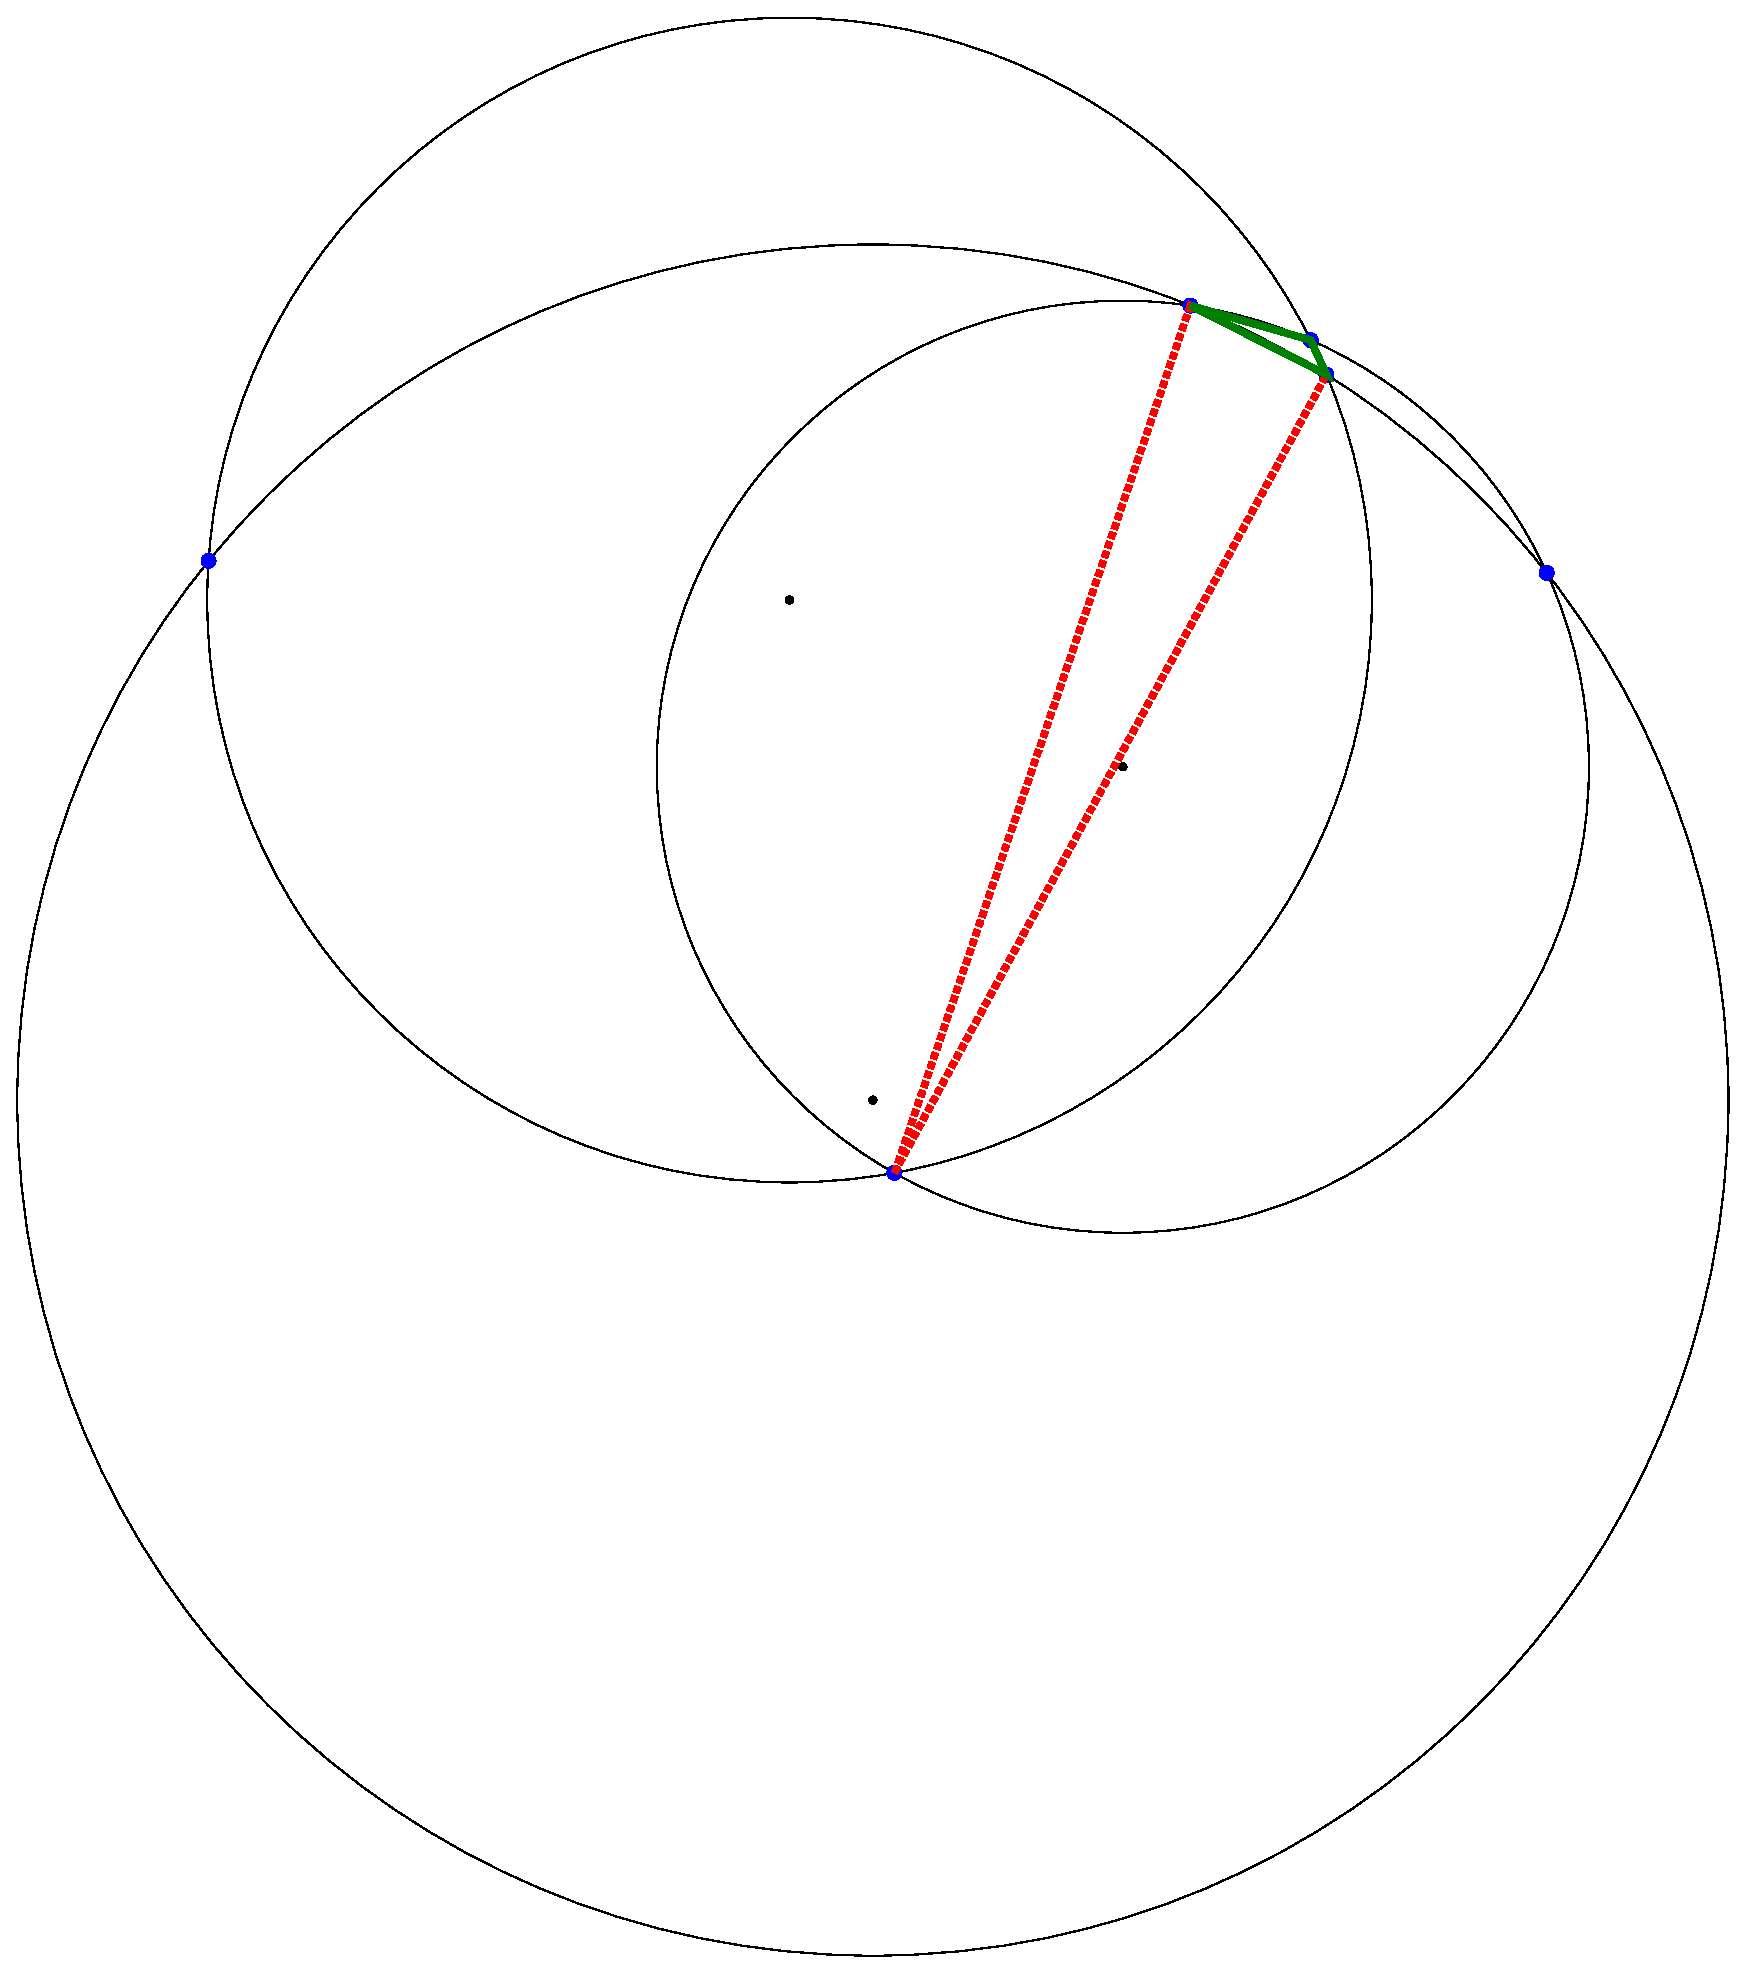
\includegraphics[width=7cm]{img/geostep3}
\end{center}
\caption{Minimum perimeter triangle and minimum triangle lying in all circles}
\label{fig:geostep3}
\end{figure}

Step 4 is again an optimization step. The algorithm detects whether the minimum perimeter triangle lies in the center of the triangle formed by the three anchors by comparing the distances of the triangles' centers of mass to the in-circle radius of the latter triangle. If it does, the center of mass of the minimum perimeter triangle is returned as the result. Afterwards, final steps 5 and 6 calculate the position estimation based on the following conditions:
\begin{itemize}
\item If the minimum perimeter triangle and the minimum perimeter triangle contained in all circles are the same or if the latter does not exist, return the geometric median of the minimum perimeter triangle's coordinates.
\item If the triangles differ, evaluate their areas: If the latter triangle's area is ``roughly equal'' to the area of the minimum perimeter triangle, return the geometric median of that triangle's coordinates.
\item If the areas are diverging more than a certain factor allows, calculate and return the geometric median of all 6 coordinates weighted by the area of their corresponding triangle.
\end{itemize}

\subsubsection{Optimizations}
Due to the many early-out conditionals in the various steps of Geo3, my attempts to vectorize the whole algorithm did not produce the desired performance gains. Instead, I decided to keep unwrapping the vectors provided by the engine at the beginning of the algorithm and only use SSE to enhance the following scalar code where possible. Apart from that, the calculation of values that remain constant over the big vector loop's iterations, namely the intersections themselves and the incircle radius of the anchor triangle, could be moved out of the loop in order to reduce redundant computation and additionally have been vectorized, using the known \texttt{circle\_get\_intersections\_v} function for all circle intersections. In the following I will explain some remarkable parts of the optimized implementation of Geo3, beginning with the precalculation of the distances between the intersection points.

\paragraph{Precalculating intersection distances.} The distances between the circle intersections are needed for both step 2 and step 3 and have priorly been calculated ad hoc when they were used, which resulted in a magnitude of wasteful computation. Therefore it seemed obvious to precalculate and store these distance values, which can be as many as 36 including symmetric and reflexive intersection pairs. This was the first time I actually had to differentiate between SSE4 and AVX coding, as the larger registers of AVX allowed for a much simpler solution than SSE did. Within the 256 bit wide \texttt{ymm} registers available on AVX-aware processors I could easily store all up to 6 intersection points and thus calculate their distance values to one of them in a single call to the vectorized \texttt{distance} function. However, since those 6 points do not fit into a 128 bit wide \texttt{xmm} register of SSE and the SSE version of the \texttt{distance} function also processes only 4 values at a time, I needed to use two registers and shuffle data around a bit in order to reduce the number of additional calls to this function, which is a rather expensive one containing several multiplications and a square root operation. See Listing~\ref{geodistances} for the code, as well as Appendix~\ref{geodistancesavx} for the AVX version. The \texttt{\_mm\_load\_ps} instructions in line 6 load the leading 4 float values from the \texttt{ix} and \texttt{iy} arrays containing the intersection points into the \texttt{\{x,y\}tlower} vectors. The SSE \texttt{MOVLHPS} instruction moves the lower two words of the second parameter register to the upper positions of the first parameter registers (i.e., \texttt{MOVLHPS((a0,a1,a2,a3), (b0,b1,b2,b3)) == (a0,a1,b0,b1))}). The intrinsic for this instruction, \texttt{\_mm\_movelh\_ps}, is used in lines 8--9 to fill the \texttt{\{x,y\}tupper} vectors with the fifth and sixth intersection point at both the lower and the upper two word positions. In other words, it simply copies the lower two words of both vectors to the corresponding upper positions. The loop starting in line 11 iterates the intersection points in steps of 2, first calculating the distances between those and the ``lower'' 4 intersection points. Then, the point vectors are merged in lines 20--21 to calculate the distances between the two points and the ``upper'' 2 intersections in a single call in line 22. This shuffling approach may seem overly complex, but in practise it achieved a performance improvement that fairly justifies the decrease in readability. This improvement mainly results from the reduced number of \texttt{distance} calls. Note that the general assumption is that in the majority of cases the algorithm has to deal with the maximum of 6 intersection points, which may become less likely with different error models. The sole purpose of the \texttt{union} declared in lines 2--5 is to provide for transparent access to the distances after SSE and AVX code paths have been joined together.

\codefile{Calculating distances for Geo3 (SSE)}{geodistances}{code/distances.c}

\paragraph{Step 2: Looking for \emph{close points}.} Having precalculated the distances between the intersection points, it is now easier to determine whether there exist 3 points which are very close together. While the previous implementation needed a nested loop to count close points for each point, in the optimization version it is sufficient to horizontally add the distance vectors for each point and test whether the sum is greater than or equal to 3. Listing~\ref{geoclosecount} shows the SSE implementation of step 2 of Geo3. The difference to the AVX version mainly consists of the extra comparison and addition operations in line 4, which are not needed for AVX as the distances reside in a single 256 bit vector, as well as a missing third horizontal add instruction. Both the fewer distance calculations and the elimination of the nested loop contributed largely to the overall performance improvement.

\codefile{Looking for 3 close points (SSE)}{geoclosecount}{code/closecount.c}

\paragraph{Step 3: Minimum perimeter triangle.} Step 3 also profitted greatly by the distance precalculation, as in order to get the triangle perimeters the original implementation computed the distances repeatedly for each possible triangle. Though, the search for the minimum perimeter triangle remains a major bottleneck in the optimized implementation. Theoretically, the algorithmic approach has a asymptotic complexity of $O(n^{3})$, since it has to process all possible 3-combinations of a set of points. Yet in practise, the implementation uses 3 nested loops with ``staggered'' initial values, i.e. the first loop starts at \texttt{i = 0}, the second loop at \texttt{j = i + 1} and so on, which, when applied to a maximum total of 6 points, results in at most 120 iterations, as compared to the theoretical maximum of $6^{3} = 216$. Trying to vectorize these loops and thus trying to access the intersection point arrays in a more sequential way would lead to the total number of tests growing closer to that maximum. Additionally, vectorization would require a lot of vector wrapping and unwrapping and data shuffling operations that will impose a significant performance overhead. Put another way, algorithms which iterate over $k$-combinations of a set of $n$ things will hardly benefit from vectorization when $n$ is small.

In short, vectorization was not an option for Geolateration's step 3. Some speed up could be achieved by vectorizing the \texttt{circle\_point\_in\_circles} function which determines whether a point lies in all circles of a given set and additionally moving this calculation out of the loop. Still, this part will continue to be a major time-consumer in Geo3. 

\paragraph{Step 5: Computing the geometric median using Weiszfeld's algorithm.} The final step of Geolateration involves calculating the geometric median of one or both of the two triangles' vertices. The geometric median (also known as Fermat-Weber point or 1-median) of a set of points is defined as the point for which the sum of the distances between this point and the points in the set becomes minimal. Since there exists no simple formula to calculate the geometric median, the authors implemented an iterative approximation approach known as Weiszfeld's algorithm~\cite{weiszfeld2009minimum}. I was able to improve the performance by deploying an SSE-enhanced version of this algorithm for up to 4 points\footnote{It is actually possible to arithmetically construct the geometric median of a triangle, which is also referred to as the \emph{Fermat point}. Since the optimized geometric median function is used exclusively for triangles in Geo3, it should probably rather have been replaced by another algorithm. I was not aware of this fact when I optimized Geo3.}, which is only used when the median of only one of the triangles needs to be calculated. For the statistically rare case when the median of two triangles should be calculated, it would be possible to translate the optimized implementation to AVX instructions, although I did not put this plan into practise. However, using SSE instructions for the two triangle case seemed inappropriate as it would require either twice as many instructions or a multitude of shuffling operations, similarly to the distance precalculation code described above. With regards to SSE programming techniques, the initial step of the algorithm is especially noteworthy, which is displayed in Listing~\ref{weiszfeld}. 

[WAS TUT EIGENTLICH weiszfeld\_test\_optimum] 

The critical point is located in lines 6--7. Considering that the distance from point (\texttt{xi},\texttt{yi}) to itself is always zero and that additionally some elements of the \texttt{ptsx} and \texttt{ptsy} vectors may also be zero as they store the user-defined parameters to the geometric median function, the elements of the \texttt{tmpx} and \texttt{tmpy} vectors may attain several special values resulting from the division operations: They may become positive infinity in case the distance value is zero and the \texttt{xi} or \texttt{yi} value is positive, negative infinity if the distance value is zero and the point value is negative, or \texttt{NaN} if both values are zero (i.e., in C, $0 / 0 = \texttt{+NaN}$). As these values must not be included in the following accumulation, they need to be detected and explicitly set to back to zero. Whereas in the original scalar implementation a conditional guarded the following code, in the SSE implementation this is accomplished using comparison instructions in lines 8--11, which assert that the \texttt{tmpx} and \texttt{tmpy} vector elements are valid floating point values between \texttt{+Inf} and \texttt{-Inf}. Note that any comparison applied to a \texttt{NaN} value always returns \texttt{false}. One may argue that the \texttt{tmpy} vector has not been checked for special values and thus may still corrupt the subsequent calculation, however, since all special cases result from a distance value (i.e., the divisor) being zero, either none or both of \texttt{tmpx} and \texttt{tmpy} may attain these special values.

\codefile{Preliminary step of the implemented 1-median algorithm}{weiszfeld}{code/weiszfeld.c}

\subsection{Algorithm III: Optimized Voting Based Location Estimation}
Like Geolateration, \emph{Optimized Voting Based Location Estimation} (VBLE-OPT) is a algorithm that has not been published by the authors yet. It is an optimized version of the \emph{Voting Based Location Estimation} algorithm proposed by Liu et al. proposed in~\cite{liu2005attackresistant}. Both algorithms project a regular grid with a defined cell length onto the playing area and vote the cells depending on whether they intersect the anchor circles. Afterwards, the algorithms recursively reduce the size of the cells and repeat the voting procedure for all highest ranked cells, until a certain minimum grid size is reached. The essential difference lies in the way the voting on cells is performed: Liu et al. defined the voted area to the anchor circle's perimeter broadened by some error threshold factor both to the outside and to the inside of the circle. Will et al., by contrast, set this circular disk to lie entirely on the outside of the circle, thereby responding to the fact that real-world distance measurements in general can only have positive errors, i.e. the measured distances will be too large rather than too short\footnote{As explained in section~\ref{ls2}, in real-world localization technologies, the distance is usually determined by measuring the round-trip time (RTT) of a signal (e.g., radio waves) travelling between the anchor node and the client. Multiplying this time with the (fixed) speed of the signal yields the estimated distance. Since obstacles (e.g., walls) in the signal's path can only decelerate its speed but not accelerate it, it is effectivly impossible to obtain too short RTTs, assuming the used clock is accurate. [ZITAT?]}. Besides, VBLE-OPT contains several optimizations that reduce the number of cells to be voted, yet these optimization do not influence the position estimation. As an illustration of the voting process, Figure~\ref{fig:vbleexample} displays two iterations of VBLE-OPT. Here, the dashed circle line represents the measured distance, i.e., the outer candidate ring. 

\begin{figure}[h]
\begin{center}
\subfigure[First iteration (section)]{
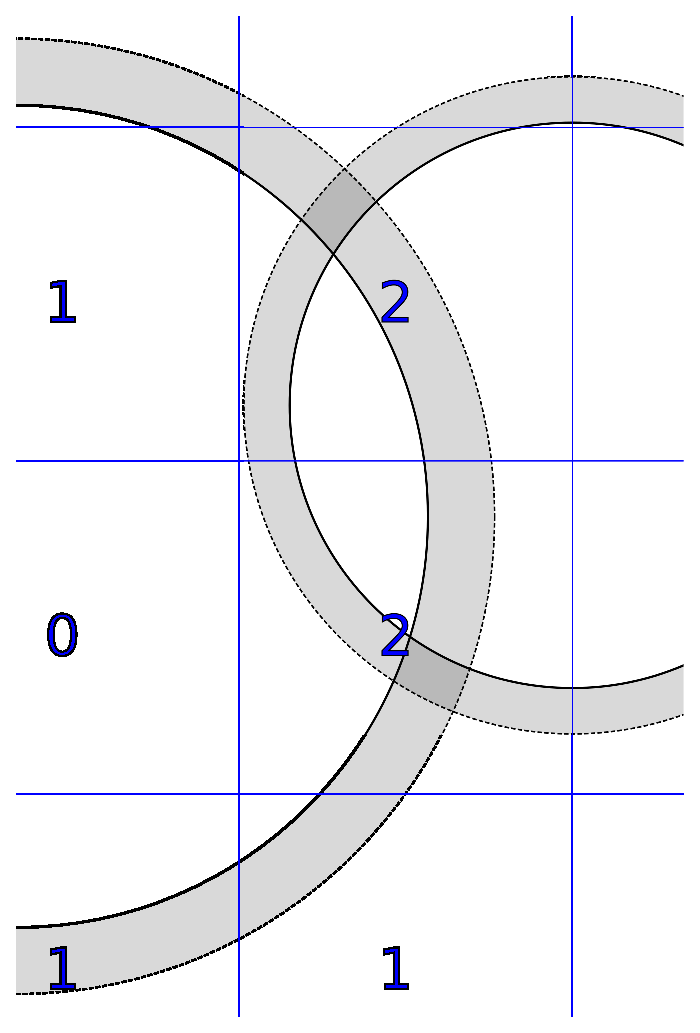
\includegraphics[width=0.4\textwidth]{img/vble.eps}
\label{fig:vble}
}
\subfigure[Second iteration]{
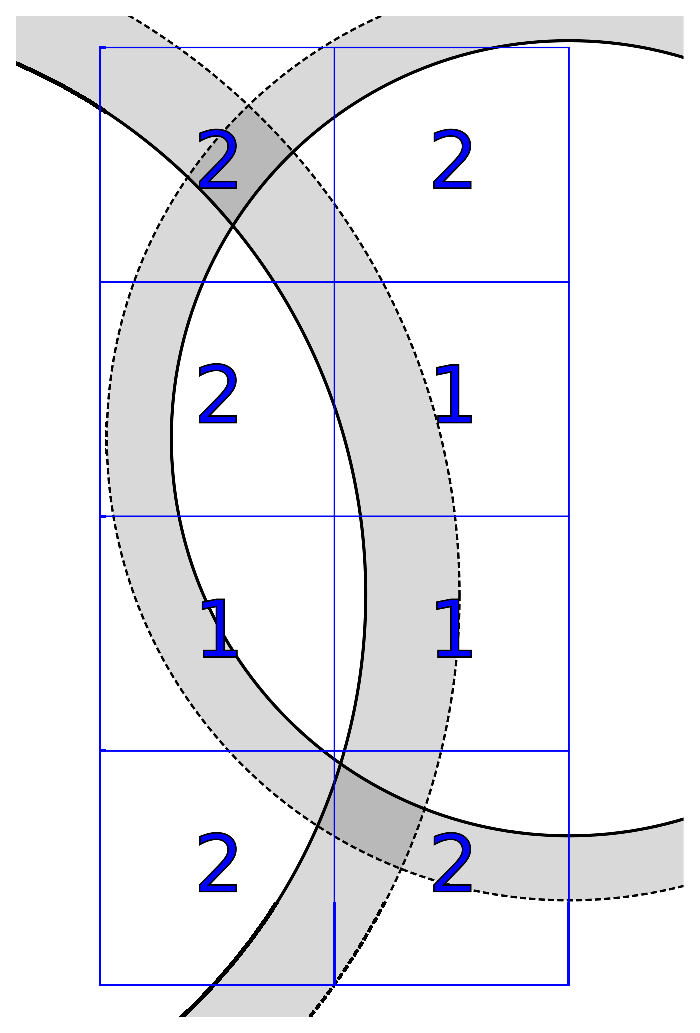
\includegraphics[width=0.4\textwidth]{img/vble2.eps}
\label{fig:vble2}
}
\end{center}
\caption{Voting example}
\label{fig:vbleexample}
\end{figure}

\subsubsection{Functionality}
As a preparative step, VBLE-OPT starts with the calculation of a minimum bounding rectangle that covers all anchors and their corresponding circles. For each anchor, the outer and inner \emph{candidate rings} are defined as circles around the anchor position that as their radii have the measured distance and this distance reduced by the error threshold, respectivly. The bounding rectangle is then divided into square cells with a side length that is initially defined as 40 per cent of the bounding rectangle's shorter side. the target cell length is defined as 5 per cent of the bounding rectangle's shorter side. The subsequent recursive main part of VBLE-OPT functions as follows:
\begin{itemize}
\item Iterating over the anchors, it first determines the outer test region of each anchor, which is the bounding box that completely covers the anchor's outer candidate ring, and the inner test region, which is defined by a number of cells that lie in the inner candidate ring but do not intersect it.
\item It then tests each cell contained in the outer test region but not in the inner test region for whether they are intersected by one of the candidate rings. For this purpose, maximum and minimum distances between the anchor position and the current cell's boundary are calculated and compared to the inner and outer radii of the candidate ring. In order to obtain these maximum and minimum distances, the algorithm determines the geometric sector of the anchor relative to the cell. See Figure~\ref{fig:vble_sector} for an illustration of the sectors. In this example, the anchor position lies in sector 8, hence the minimum distance is to be found between the anchor and the bottom side of the cell, whereas the maximum distance is between the anchor and the upper left corner.
\item If the cell is intersected by one of the candidate rings, its voting score is incremented. Along the way, the algorithm keeps track of the current maximum score as well as the bounding rectangle that covers all cells that have been voted that score.
\item After all anchors have been processed, the bounding rectangle containing all highest-ranked cells is used as the playing area of the following iteration, with the cells' side length being halved.
\end{itemize}

\begin{figure}
\begin{center}
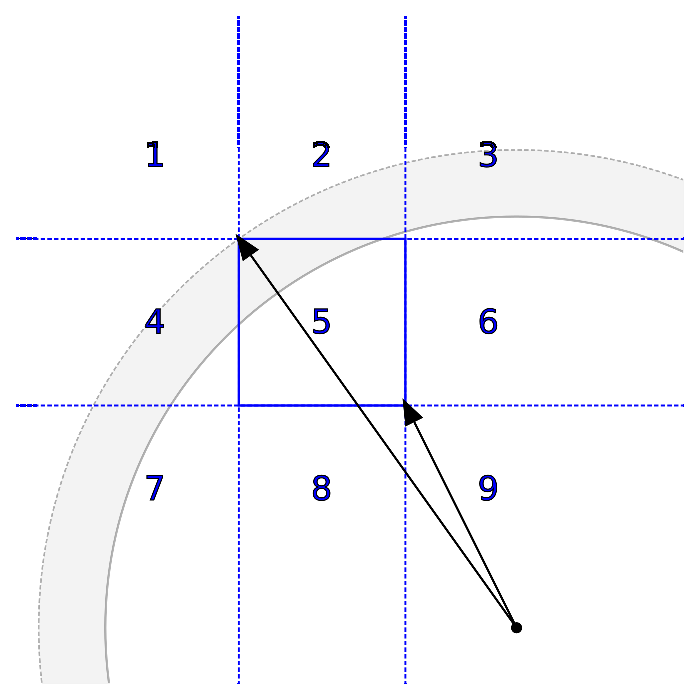
\includegraphics[width=0.4\textwidth]{img/vble_sector.eps}
\end{center}
\caption{Sector determination}
\label{fig:vble_sector}
\end{figure}

When the grid has reached the desired granularity, the centers of the highest-scored cells are accumulated and their center of mass is returned as the position estimation. For reference, the basic outline of the algorithm is shown in Listing~\ref{vbleopt_outline}.

\codefile{Outline of the VBLE-OPT algorithm}{vbleopt_outline}{code/vble_outline.c}

\subsubsection{Optimizations}
Despite its apparent simplicity, the VBLE-OPT algorithm was difficult to optimize due to its many code paths and irregular performing. For example, in the algorithm's inner two loops, which iterate over the cells to be voted on by their x- and y-coordinate, the loop counters are bounded by the calculated outer test region. Additionally, the inner-most loop may be cancelled by a \texttt{break} statement in case the current cell is covered by the inner test region. It is therefore hardly possible to know the number of iterations of these loops for a particular anchor beforehand, and it is also doubtful that this number is similar over multiple runs of the algorithm (i.e., multiple distance measurements for the same anchor). As a result, although most of the loop body can be vectorized easily, a number of blacklists need to be maintained in order to reflect the varying number of loop iterations.

\paragraph{Complete vectorization.} 
These blacklists indicate whether a vector element (i.e., a run of the algorithm) has already passed the loop limits, in other words, whether its whole test region has already been processed. Fortunately, since the main portion of code contained in the loop body has no outside effects, the blacklists need to be examined only before updating the voting scores. My first attempt at optimizing VBLE-OPT consisted of a major rewrite of the algorithm that targeted at vectorizing it as a whole. I used SSE4 integer intrinsics to manipulate the loop counters in parallel. As a consequence, this prevents the implementation to make use of the AVX unit of recent processors, as AVX does not include integer instructions until now. Listing~\ref{vble_vectorized} displays an extract from the vectorized implementation of VBLE-OPT.

\codefile{Simplified code of the vectorized implementation of VBLE-OPT}{vble_vectorized}{code/vble_vectorized.c}

Line 7 shows the creation of the first blacklist, which masks vector elements for which the loop counter \texttt{j} has already passed the corresponding \texttt{xMax} limit. The \texttt{\_mm\_cvtepi32\_ps} instruction, which converts 4 packed integer values stored in an \texttt{xmm} register into 4 packed floats, fills the gap for the integer ``greater or equal'' comparison instruction that is still missing in SSE4. Lines 23--33 mark the voting procedure of VBLE-OPT: First, the array indices of the current cells are calculated using vector operations such as \texttt{\_mm\_mullo\_epi32}, which multiplies two \texttt{xmm} registers filled with 4 signed integers. Based on the calculated minimum and maximum distances and the candidate ring (\texttt{anchor[i].ri} and \texttt{anchor[i].ro}), it is then decided which of the current cells should be voted for (l. 27). In line 28, the voting score increment of these cells is set to 1, but only if they were not blacklisted before in which case it is set to zero. Finally, the score of each cell is updated. The latter also constitutes one of the major bottlenecks of the implementation, since the \texttt{scores} array needs to be accessed in a nonparallel and totally random way.

Not shown in Listing~\ref{vble_vectorized} is a lengthy code section that determines the anchor's sector relative to the cells, which is necessary for calculating the anchor's minimum and maximum distance to the cell boundary (refer to Figure~\ref{fig:vble_sector}). The original implementation contained a long sequence of conditional statements, that determined the sector by comparing the anchor's coordinates to the corner points of the current cell. In the SSE implementation, I replaced these conditionals with a series of \texttt{blendvps} instructions, that blended the distances to the \texttt{dMax} and \texttt{dMin} vectors based on the results of a large number of vector comparisons. Additionally, since the original code left the sector determination once the proper sector was found (using a chain of \texttt{if-else-if-...} statements), it was necessary to maintain a bitmask that indicated which vector elements have been successfully processed and incorporate this bitmask into the blending instructions. In sum, the vectorized implementation unconditionally calculated every possible distance value, used plenty of comparisons and \texttt{blendvps} instructions, and required additional logical operations for maintaining the bitmask. By contrast, the scalar implementation required only a minimum number of arithmetic operations and up to 9 comparisons, in addition to a conditional jump. In the end, my initial approach at vectorizing VBLE-OPT turned out to perform about 1.5 times slower than the original implementation.

\paragraph{Minor optimizations.}
As a consequence of this initial failure, I started over with a clean version of the original code, this time trying to optimize smaller, isolated parts of the algorithm. The implementation, showing much potential for code restructuring and better memory management, was benefitted by the following measures:
\begin{itemize}
\item The voting array was (probably as a reminiscence to C89, where arrays of dynamic size could not be allocated on the stack) dynamically allocated using \texttt{malloc}. Changing this to stack allocation measurably improved performance.
\item Several constant values were repeatedly calculated in the inner loops. I modified the implementation to precalculate these values (e.g., the candidate rings of the anchors and the inner test region) in advance.
\item To test whether a cell is overlapped by a candidate ring, the original implementation used euclidean distances. In order to save several square root instructions, I changed this to use squared euclidean distances instead.
\item As a remarkable example of the \emph{locality of reference} principle, I introduced the \texttt{anchor\_info\_t} struct that contains the coordinates of an anchor as well as its candidate ring and inner test region and thus keeps these values close together in memory. Since the anchors are processed iterativly, this considerably reduced the number of cache misses in the inner loops.
\item For final position estimation, the original implementation calculated the center of mass of the centers of the highest-ranked cells. In order to calculate these center positions, it added half of the grid cells' side length to the cells' coordinates, which point to the top-left corner of the cells. I deferred this ``centering'' until after the center of mass has been calculated, thereby saving a number of addition operations.
\end{itemize}
These combined measures led to a moderate improvement of the overall performance of the algorithm. However, the breakthrough results I had expected failed to materialize.

\paragraph{Sector determination.}
Later, while trying to reduce the number of branch mispredictions resulting from conditionals contained in the sector determination section, I found a mathematical approach to calculate the minimum and maximum distances that does not require any conditional statements. Although this again is an algorithmic optimization, I decided to include it in the algorithm as it drastically improved performance. Since it is not obvious to understand from the code (see Listing~\ref{sectors}), I will give a brief explanation of this approach in the following, for later reference.

First, we need to calculate the point on the cell boundary that is closest to the anchor. This is a simple matter of ``clamping'' the anchor coordinates to the cell's vertical and horizontal extents, where clamping is defined as \texttt{clamp(v, min, max) = (v < min) ? min : ((v > max) ? max : v)}. Afterwards, we use vector mathematics to reach the most distance point, i.e. we travel along the longer section of the cell side that the closest point lies on and travel an entire cell side in the orthogonal direction (ll. 6--7). In lines 7--8 we construct the vector pointing to the closest point, however, since the \texttt{farXoffset} and \texttt{farYoffset} values are always positive, we mirror it onto the first quadrant by using absolute values (where figuratively the anchor is the coordinate system's origin). The vector pointing to the most-distant point is created by adding the offsets to the closest point vector (ll. 10--11). Finally, the squared euclidean distances are calculated in lines 12--13.

After I discovered this alternate solution to the minimum/maximum distance problem, I embedded it into the initial fully-vectorized implementation. Unexpectedly, this resulted in a significant performance gain, up to the point where this version largely outperformed the optimized scalar implementation. The final optimized version consists of the vectorized implementation enhanced with the smaller optimizations mentioned above. However, the achieved speed-up relies on the similarity of the input parameters provided by the engine. My experiments suggest that in the majority of cases, the number of loop iterations in the main loop is constant over all vector elements. This again may change with other error models being added to LS$^{2}$.

\codefile{Sector determination using vector mathematics}{sectors}{code/sectors.c}
